\documentclass[a4paper, 12pt]{scrartcl}

\usepackage{math-practice}

\area{Lineáris algebra}
\title{Lineáris egyenletrendszerek}
\subject{Matematika G2}
\subjectCode{BMETE94BG02}
\date{Utoljára frissítve: \today}
\docno{3}

\begin{document}
\maketitle
\subsection{Elméleti Áttekintő}

\begin{blueBox}
  Az $m$ egyenletből és $n$ ismeretlenből álló lineáris egyenletrendszer
  általános alakja:
  $$
    \begin{array}{*{9}{c}}
      a_{11} x_{1} & + & a_{12} x_{2} & + & \dots  & + & a_{1n} x_{n} & = & b_{1}\text, \\
      a_{21} x_{1} & + & a_{22} x_{2} & + & \dots  & + & a_{2n} x_{n} & = & b_{2}\text, \\
      \vdots       &   & \vdots       &   & \vdots &   & \vdots       &   & \vdots      \\
      a_{m1} x_{1} & + & a_{m2} x_{2} & + & \dots  & + & a_{mn} x_{n} & = & b_{m}\text,
    \end{array}
  $$
  ahol $a_{ij}$ az együtthatókat, $b_{j}$ a konstansokat, $x_{j}$ pedig az
  ismeretleneket jelöli.

  Egy lineáris egyenletrendszer felírható $\rmat A \rvec x = \rmat b$
  alakban, ahol $\rmat A$ az együttható mátrix, $\rvec x$ az ismeretlenek
  vektora, $\rvec b$ pedig a konstans vektor.
  $$
    \underbrace{\begin{bmatrix}
        a_{11} & a_{12} & \cdots & a_{1n} \\
        a_{21} & a_{22} & \cdots & a_{2n} \\
        \vdots & \vdots & \ddots & \vdots \\
        a_{m1} & a_{m2} & \cdots & a_{mn}
      \end{bmatrix}}_{\rmat A} \underbrace{\begin{bmatrix}
        x_{1} \\ x_{2} \\ \vdots \\ x_{n}
      \end{bmatrix}}_{\rvec x} = \underbrace{\begin{bmatrix}
        b_{1} \\ b_{2} \\ \vdots \\ b_{n}
      \end{bmatrix}}_{\rvec b}
  $$
\end{blueBox}

\begin{theorem}[LER megoldhatóságának szükséges és elégséges feltétele]
  Az $\rmat A \rvec x = \rvec b$ lineáris egyenletrendszer akkor és csak
  akkor oldható meg, ha $\rg(\rmat A) = \rg(\rmat A | \rvec b)$, ahol az
  $(\rmat A | \rvec b)$ mátrixot kibővített mátrixnak nevezzük.

  A feltétel mátrixosan:
  $$
    \rg \begin{bmatrix}
      a_{11} & a_{12} & \cdots & a_{1n} \\
      a_{21} & a_{22} & \cdots & a_{2n} \\
      \vdots & \vdots & \ddots & \vdots \\
      a_{m1} & a_{m2} & \cdots & a_{mn}
    \end{bmatrix} = \rg \left[\begin{array}{cccc|c}
        a_{11} & a_{12} & \cdots & a_{1n} & b_1    \\
        a_{21} & a_{22} & \cdots & a_{2n} & b_2    \\
        \vdots & \vdots & \ddots & \vdots & \vdots \\
        a_{m1} & a_{m2} & \cdots & a_{mn} & b_n
      \end{array}\right]\text.
  $$
\end{theorem}

\begin{definition}[Homogén lineáris egyenletrendszer]
  Az $\rmat A \rvec x = \rvec b$ lineáris egyenletrendszer homogénnek mondjuk,
  ha $\rvec b = \nvec$.

  Ha $\rvec b \neq \nvec$, akkor a lineáris egyenletrendszer inhomogén.
\end{definition}

\begin{note}
  A feltételből következik, hogy homogén lineáris egyenletrendszer
  ($\rvec b = \nvec$) mindig megoldható, hiszen az együttható mátrixból és egy
  nullvektorból képzett kibővített mátrix rangja mindig meg fog egyezni az
  együttható mátrix rangjával.
\end{note}

\begin{blueBox}
  \sftitle{Lineáris egyenletrendszer csoportosítása:}

  \begin{itemize}
    \item A LER \textbf{megoldható}, ha létezik megoldása.

    \item A LER \textbf{ellentmondó}, ha nincs megoldása.

    \item A LER \textbf{határozott}, ha csupán egyetlen megoldása van.

    \item A LER \textbf{határozatlan}, ha végtelen sok megoldása van.
  \end{itemize}
\end{blueBox}

\begin{blueBox}
  \sftitle{A megoldások vizsgálata:}

  Megoldás akkor létetik, ha $\rvec b$ előállítható $\rmat A$ oszlopvektorainak
  lineáris kombinációjaként, azaz ha $\rg \rmat A = \rg (\rmat A | \rvec b)$.

  Ha $\rg \rmat A \neq \rg (\rmat A | \rvec b)$, akkor az egyenletrendszernek
  nincs megoldása.

  Ha $\rg A < n$, vagyis az együttható mátrix rangja kisebb, mint az
  ismeretlenek száma, akkor az egyenletrendszernek végtelen sok
  megoldása van. Az $\rmat A$ mátrix rangja segítségével meghatározható,
  hogy hány paramétert kell bevezetnünk a megoldás megadásához:
  $$
    p = n - \rg \rmat A
    \text{, ahol $p$ a paraméterek száma.}
  $$
\end{blueBox}

\begin{blueBox}
  \sftitle{Megoldási módszerek}:

  \begin{enumerate}
    \item \textbf{Mátrixinverz módszer}: ha az $\rmat A$ mátrix reguláris, akkor
          invertálható és $\rvec x = \rmat A^{-1} \rvec b$.

    \item \textbf{Cramer-szabály}: ha az $\rmat A$ mátrix reguláris, akkor az
          együtthatók az alábbi módon számíthatóak:
          $$
            x_i = \frac{\det \rmat A_i}{\det \rmat A}
            \text,
          $$
          ahol az $\rmat A_i$ mátrixot úgy képezzük, hogy az $i$-edik oszlopába
          $\rvec b$ vektort írjuk be.

    \item \textbf{Gauss-elimináció}: elemi átalakításokkal (sorműveletekkel)
          átalakítjuk a kibővített mátrixot.
          $$
            \left[\begin{array}{cccc|c}
                a_{11} & a_{12} & \cdots & a_{1n} & b_1    \\
                a_{21} & a_{22} & \cdots & a_{2n} & b_2    \\
                \vdots & \vdots & \ddots & \vdots & \vdots \\
                a_{m1} & a_{m2} & \cdots & a_{mn} & b_n
              \end{array}\right]
            \quad\sim\quad
            \left[\begin{array}{cccc|c}
                \square & \square & \cdots & \square & \square \\
                0       & \square & \cdots & \square & \square \\
                \vdots  & \vdots  & \ddots & \vdots  & \vdots  \\
                0       & 0       & \cdots & \circ   & \circ
              \end{array}\right]
          $$

          Célunk: felső háromszögmátrix alakra hozni a kibővített mátrixot.

          A megoldások száma:
          \begin{center}
            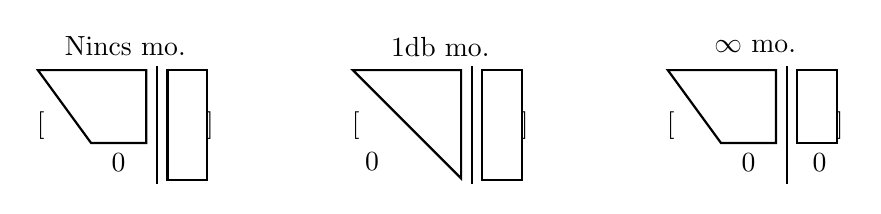
\begin{tikzpicture}[thick]
              \foreach \i in {0,1,2} {
                  \node at (\i*4cm,0) {$\left[\phantom{\begin{matrix}10000000000\\\\\\\\\end{matrix}}\right]$};

                  \draw (\i*4cm+4mm,.75cm) -- ++(0,-1.5cm);
                }

              \draw (5.35mm,7mm) rectangle ++(5mm, -14mm);
              \draw (45.35mm,7mm) rectangle ++(5mm, -14mm);
              \draw (85.35mm,7mm) rectangle ++(5mm, -9.25mm) node[below left] {$0$};

              \draw (2.65mm,7mm)
              -- ++(-13.75mm,0)
              -- ++(6.75mm,-9.25mm)
              -- ++(7mm,0)
              node[midway, below] {$0$}
              -- cycle;
              \draw (42.65mm,7mm)
              -- ++(-13.75mm,0)
              -- ++(13.75mm,-13.75mm)
              node[midway, below left=2.25mm] {$\quad0$}
              -- cycle;
              \draw (82.65mm,7mm)
              -- ++(-13.75mm,0)
              -- ++(6.75mm,-9.25mm)
              -- ++(7mm,0)
              node[midway, below] {$0$}
              -- cycle;

              \node[] at (0cm,1cm) {Nincs mo.};
              \node[] at (4cm,1cm) {1db mo.};
              \node[] at (8cm,1cm) {$\infty$ mo.};
            \end{tikzpicture}
          \end{center}
  \end{enumerate}
\end{blueBox}

\clearpage
\subsection{Feladatok}

\begin{enumerate}

  \item Adott egy lineáris egyenletrendszer $\textbf{A}$ mátrix típusa, rangja,
        illetve a kibővített mátrix rangja. Határozza meg az egyenletrendszer
        megoldásainak számát!
        $$
          \begin{array}{|c|c|c|}
            \hline
            \rmat A  & \rg \rmat A & \rg(\rmat A | \rvec b) \\
            \hline
            4\times3 & 3           & 4                      \\
            \hline
            3\times3 & 2           & 2                      \\
            \hline
            6\times8 & 6           & 6                      \\
            \hline
            8\times6 & 6           & 6                      \\
            \hline
            3\times2 & 0           & 0                      \\
            \hline
          \end{array}
        $$

  \item Oldja meg az alábbi lineáris egyenletrendszert mátrixinverz módszerrel!
        $$
          \begin{aligned}
            x_1 + 3x_2 + 3x_3 & = 3 \\
            x_1 + 3x_2 + 4x_3 & = 6 \\
            x_1 + 4x_2 + 3x_3 & = 9
          \end{aligned}
        $$

  \item Vezesse vissza az alábbi egyenletet lineáris egyenletrendszerre, majd
        oldja meg mátrixinverz módszerrel!
        $$
          \rmat A = \begin{bmatrix}
            1  & 2 \\
            -2 & 3
          \end{bmatrix}
          \qquad
          \rmat B = \begin{bmatrix}
            5 \\
            1
          \end{bmatrix}
          \qquad
          \rmat A \rvec x = \rmat B + 2 \rvec x
        $$

  \item Cramer-szabály segítségével oldja meg az alábbi lineáris
        egyenletrendszert!
        $$
          \left\{\;
          \begin{aligned}
            2x_1 - 3x_2 + x_3   & = 0  \\
            -3x_1 + 4x_2 - 2x_3 & = 1  \\
            5x_1 + 4x_3         & = -3
          \end{aligned}
          \right.
        $$

  \item Határozza meg $x_1 - x_2$ értékét!
        $$
          \left\{\;
          \begin{aligned}
            x_1 + 2x_2 + 3x_3 + 4x_4 & = 5  \\
            2x_1 + x_2 + 2x_3 + 3x_4 & = 1  \\
            3x_1 + 2x_2 + x_3 + 2x_4 & = 1  \\
            4x_1 + 3x_2 + 2x_3 + x_4 & = -5
          \end{aligned}
          \right.
        $$

  \item Oldja meg az alábbi lineáris egyenletrendszert Gauss-eliminációval!
        $$
          \left\{\;
          \begin{aligned}
            x_1 + 2x_2 - x_3  & = 2  \\
            3x_1 - x_2 + 2x_3 & = 7  \\
            x_1 - x_3         & = -2 \\
            2x_1 + x_2 + x_3  & = 7
          \end{aligned}
          \right.
        $$

  \item Oldja meg az alábbi lineáris egyenletrendszert Gauss-eliminációval!
        $$
          \left\{\;
          \begin{aligned}
            5x_1 - x_2 + 2x_3 + x_4  & = 7 \\
            2x_1 + x_2 + 4x_3 - 2x_4 & = 1 \\
            x_1 - 3x_2 - 6x_3 + 5x_4 & = 0
          \end{aligned}
          \right.
        $$

  \item Oldja meg azt a lineáris egyenletrendszert, melynek a kibővített mátrixa
        $(\rmat A | \rvec b)$ alakú!
        $$
          (\rmat A | \rvec b) =
          \left[
            \begin{matrix}
              1  & 1  & 1  & 2  & 1 \\
              -2 & -2 & -6 & -8 & 0 \\
              2  & 2  & -3 & -1 & 4 \\
              -1 & -1 & 1  & 0  & 4 \\
              3  & 3  & 6  & 9  & 8 \\
            \end{matrix}
            \;\middle|\;
            \begin{matrix}
              2  \\
              10 \\
              17 \\
              9  \\
              15
            \end{matrix}
          \right]
        $$

  \item Oldja meg az alábbi lineáris egyenletrendszert Gauss-eliminációval:
        $$
          \left\{\;
          \begin{aligned}
            x_1 + 3x_2 + 2x_3  & = 0 \\
            2x_1 - x_2 + 3x_3  & = 0 \\
            3x_1 - 5x_2 + 4x_3 & = 0 \\
            x_1 + 17x_2 + 4x_3 & = 0
          \end{aligned}
          \right.
        $$

  \item Oldja meg azt a homogén lineáris egyenletrendszert, amelynek a
        együtthatóit az $\rmat A$ mátrix tartalmazza!
        $$
          \rmat A =
          \begin{bmatrix}
            1 & 1 & -4 \\
            4 & 7 & 5  \\
            3 & 5 & 2  \\
            2 & 9 & 6
          \end{bmatrix}
        $$

  \item Az egyenletrendszer megoldása nélkül állapítsa meg, hogy csak a
        triviális megoldás létezik, vagy van nem triviális megoldás is!
        $$
          \left\{\;
          \begin{aligned}
            2x_1 + x_2 - 4x_3  & = 0 \\
            3x_1 + 5x_2 - 7x_3 & = 0 \\
            4x_1 - 5x_2 + 6x_3 & = 0
          \end{aligned}
          \right.
        $$

  \item Adja meg $C$ értékét, hogy megoldható legyen az egyenletrendszer!
        $$
          \left\{\;
          \begin{aligned}
            x_1 + 2x_2 - 3x_3 + x_4   & = 2 \\
            2x_1 + 3x_2 - 3x_3 - 2x_4 & = 4 \\
            -3x_1 - 5x_2 + 4x_3 + x_4 & = C
          \end{aligned}
          \right.
        $$

  \item Az egyenletrendszer megoldása nélkül állapítsa meg, hogy csak a
        triviális megoldás létezik, vagy van nem triviális megoldás is!
        $$
          \left\{\;
          \begin{aligned}
            x_1 + 2x_2 + 3x_3 + 4x_4 + 5x_5 & = 0 \\
            -x_1 + x_2 - 6x_4 + x_5         & = 0 \\
            3x_2 + x_3 + 5x_4 - x_5         & = 0 \\
            2x_3 - 7x_4 + 6x_5              & = 0
          \end{aligned}
          \right.
        $$

  \item Az $u$ és $v$ paraméterek függvényében hány megoldása van az
        egyenletrendszernek, ha a kibővített mátrix $(\rmat A | \rvec b)$ alakú?
        $$
          (\rmat A | \rvec b) =
          \left[
            \begin{matrix}
              3 & 5 & -1 \\
              1 & u & 2  \\
              1 & 9 & -5 \\
            \end{matrix}
            \;\middle|\;
            \begin{matrix}
              1 \\
              2 \\
              v \\
            \end{matrix}
          \right]
        $$
\end{enumerate}
\end{document}